\chapter{Introduction}
\label{chap:introduction}

An always-on robot can watch a room for days, remember what happened in it and learn when it tends to be busy, and still behave exactly as it did on the first morning. The always-on cognitive architecture developed for the iCub by \citet{Pasquali2024ArtificialCognition,Pasquali2025AlwaysOn} is such a robot. It segments a continuous audiovisual stream into episodes, stores them in an associative memory and recognises recurring social contexts without supervision. Its behaviour module, however, keeps tracking faces and otherwise wandering its gaze, whatever the memory has learned. Its authors name the two missing pieces themselves: an action-selection loop that turns recognition into action, and a value system that defines what matters to the robot and why \citep{Pasquali2025AlwaysOn,Pasquali2026ISEED}.

This thesis builds the first and supplies one example of the second. An embodied behaviour architecture replaces the inherited behaviour module and lets the robot's internal state change whom it looks at, whom it approaches and what it says. The value installed on it is a synthetic orexigenic (appetite-stimulating) drive: an energy reserve that drains over time and with every social act, and that only the people nearby can refill. Energy maintenance, which robots usually leave to a docking station or an operator, becomes part of the social exchange.

\section[The always-on cognitive architecture inherited by this thesis]{The always-on cognitive architecture\\inherited by this thesis}
\label{sec:intro-developmental-architecture}

The inherited architecture comes from a research programme begun in \emph{Artificial Cognition, from the Ground Up} \citep{Pasquali2024ArtificialCognition} and extended in \emph{No Robot Is an Island} \citep{Pasquali2025AlwaysOn}. In its latest form, named iSEED (Interaction-oriented Situated Embodied Experience-Driven), this \emph{always-on cognitive architecture} rests on three pillars, embodiment, memory and values, and is meant as a minimal testbed for how artificial cognition first emerges, not as a complete system \citep{Pasquali2026ISEED}. The agent has no explicit task. A curiosity-like proto-motivation turns it toward whatever departs from what it has recently perceived, since such departures may mark socially meaningful events. Where most current robotics relies on deep learning and large language models trained offline on large generic datasets \citep{Pasquali2025AlwaysOn}, the programme follows an \emph{emergent enactive} methodology \citep{Pasquali2024ArtificialCognition,Sandini2025MutualUnderstanding}: cognitive ability develops through the agent's own interaction with its environment instead of being built in beforehand.

\begin{figure}[H]
    \centering
    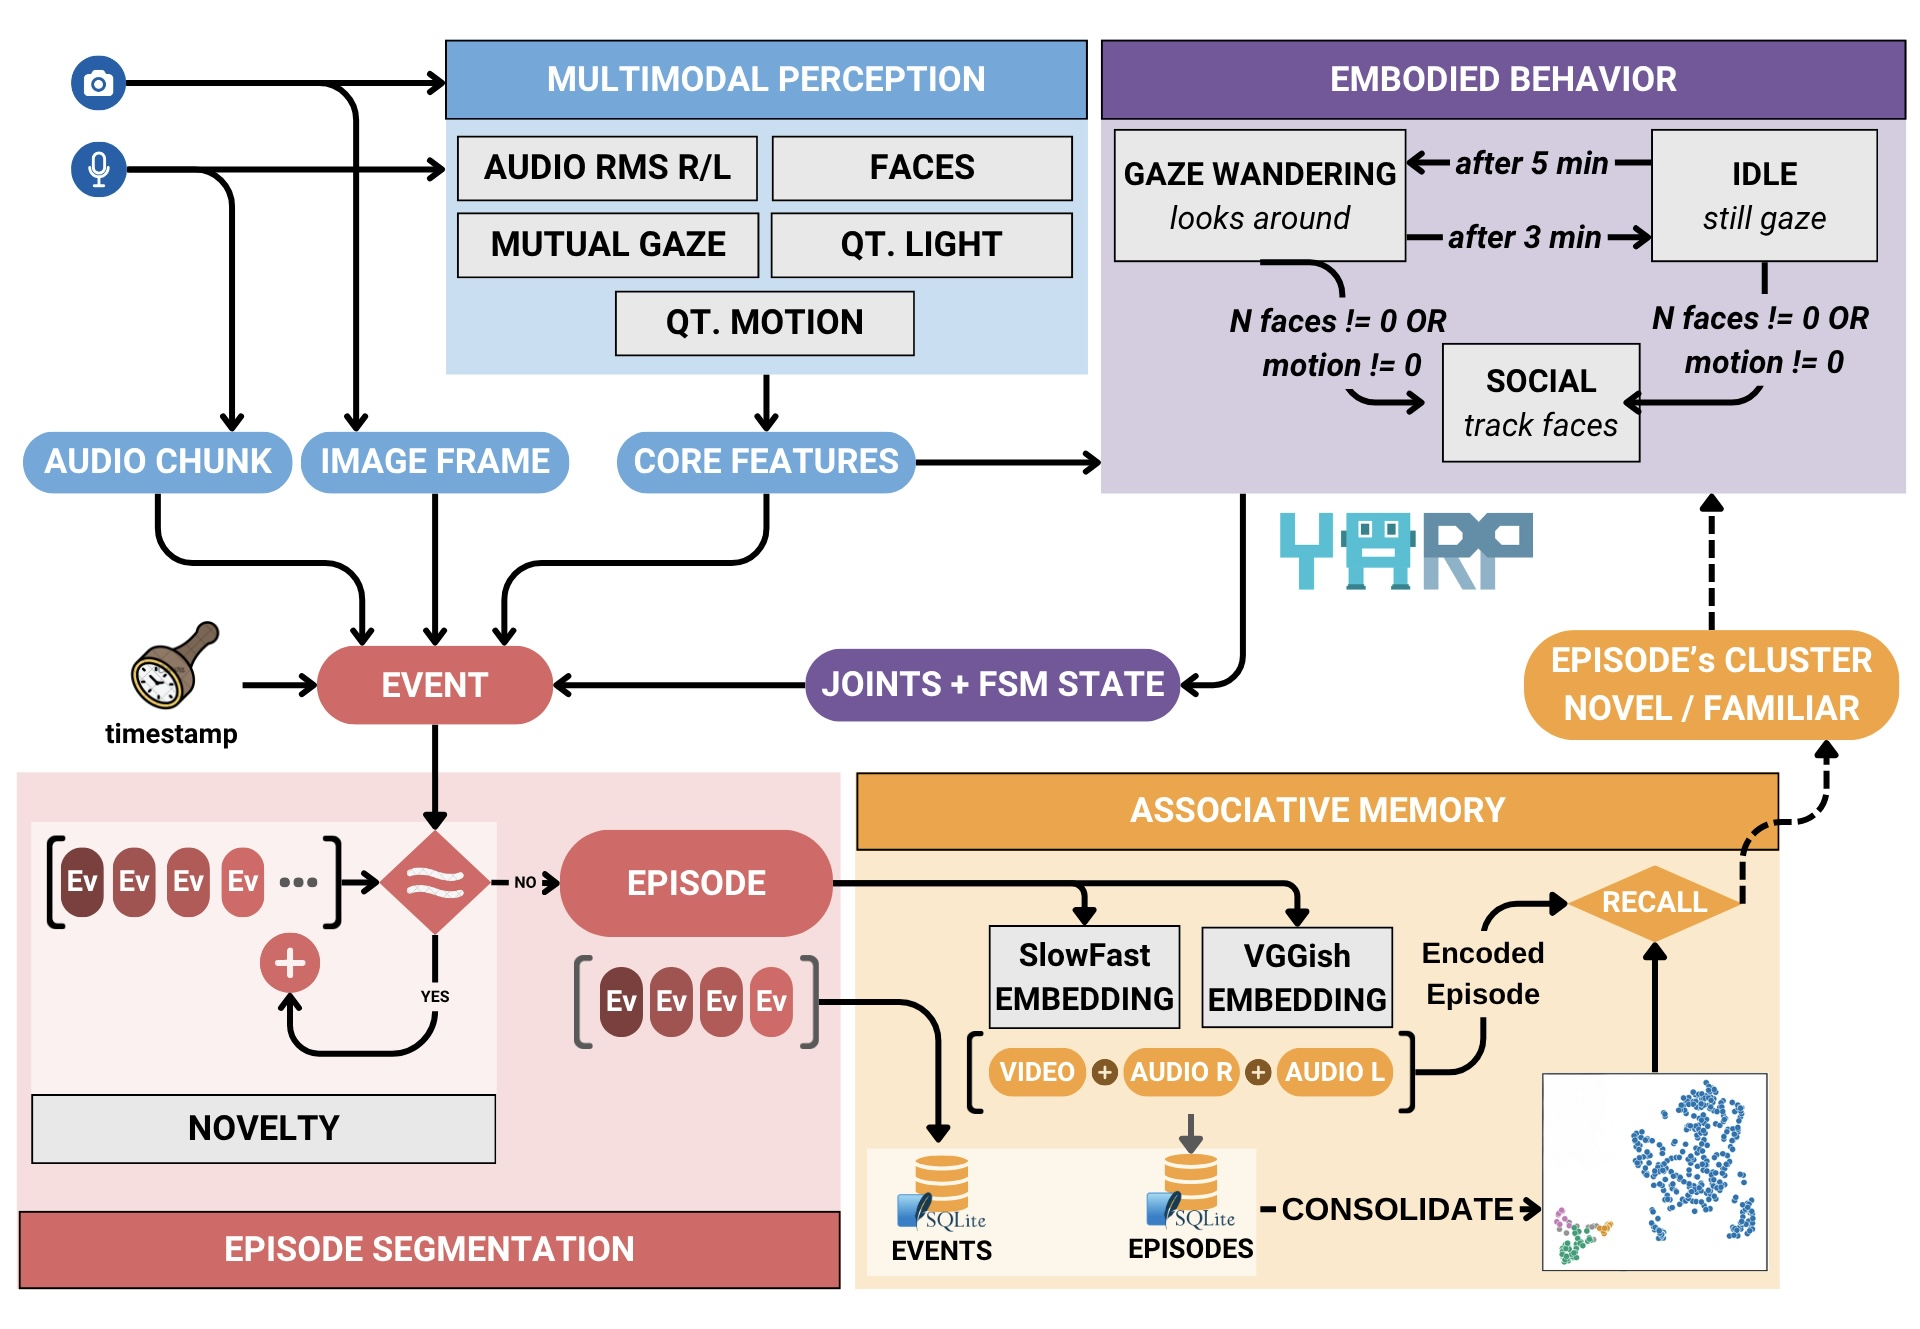
\includegraphics[width=0.88\textwidth,height=0.38\textheight,keepaspectratio]{Introduction/Figures/always-on-architecture.jpg}
    \caption[Always-on cognitive architecture.]{Always-on cognitive architecture inherited by this thesis \citep{Pasquali2025AlwaysOn}. The diagram shows the original configuration with the SlowFast video encoder: multimodal perception and embodied behaviour contribute to event formation, episode segmentation detects novelty, and associative memory encodes and consolidates experience before returning a familiar or novel cluster assignment.}
    \label{fig:pasquali-always-on-architecture}
\end{figure}

\citet{Pasquali2026ISEED} adopt the definition of cognition by \citet{Vernon2014Artificial}: ``the process by which an autonomous system perceives its environment, learns from experience, anticipates the outcome of events, acts to pursue goals, and adapts to changing circumstances''. It starts from a few innate (phylogenetic) abilities, not hand-crafted symbolic rules, and builds its own (ontogenetic) knowledge from experience. That knowledge serves one aim, internal consistency: keeping what the agent expects in line with what it perceives. It is also \emph{altricial}: like a human infant, it depends on other social agents to develop, not on its own competences alone \citep{Sloman2005Altricial,Pasquali2026ISEED}. The caregiver-mediated loop built in this thesis rests on that condition.

Rather than a single perception--action cycle, \citet{Pasquali2026ISEED} model cognition as several coupled dynamical loops running in parallel (Figure~\ref{fig:pasquali-iseed-loops}). Body and environment close one loop through overt action and perception, a body model and motivational dynamics another through covert action, internal simulation and sensory prediction. Where dual-process accounts fix the number of processing systems at two, \citet{Pasquali2026ISEED} hypothesise that a cognitive agent's foundational ability is to generate, sustain, close and make sense of such loops, which development extends across bodily, physical, social and temporal horizons. The architecture they validated filled only the lower loop: perception and overt gaze were in place and memory supplied temporal depth, but the motivational dynamics of the upper loop had no implementation and no path back to action. This thesis builds that path and gives the upper loop its first value.

\begin{figure}[H]
    \centering
    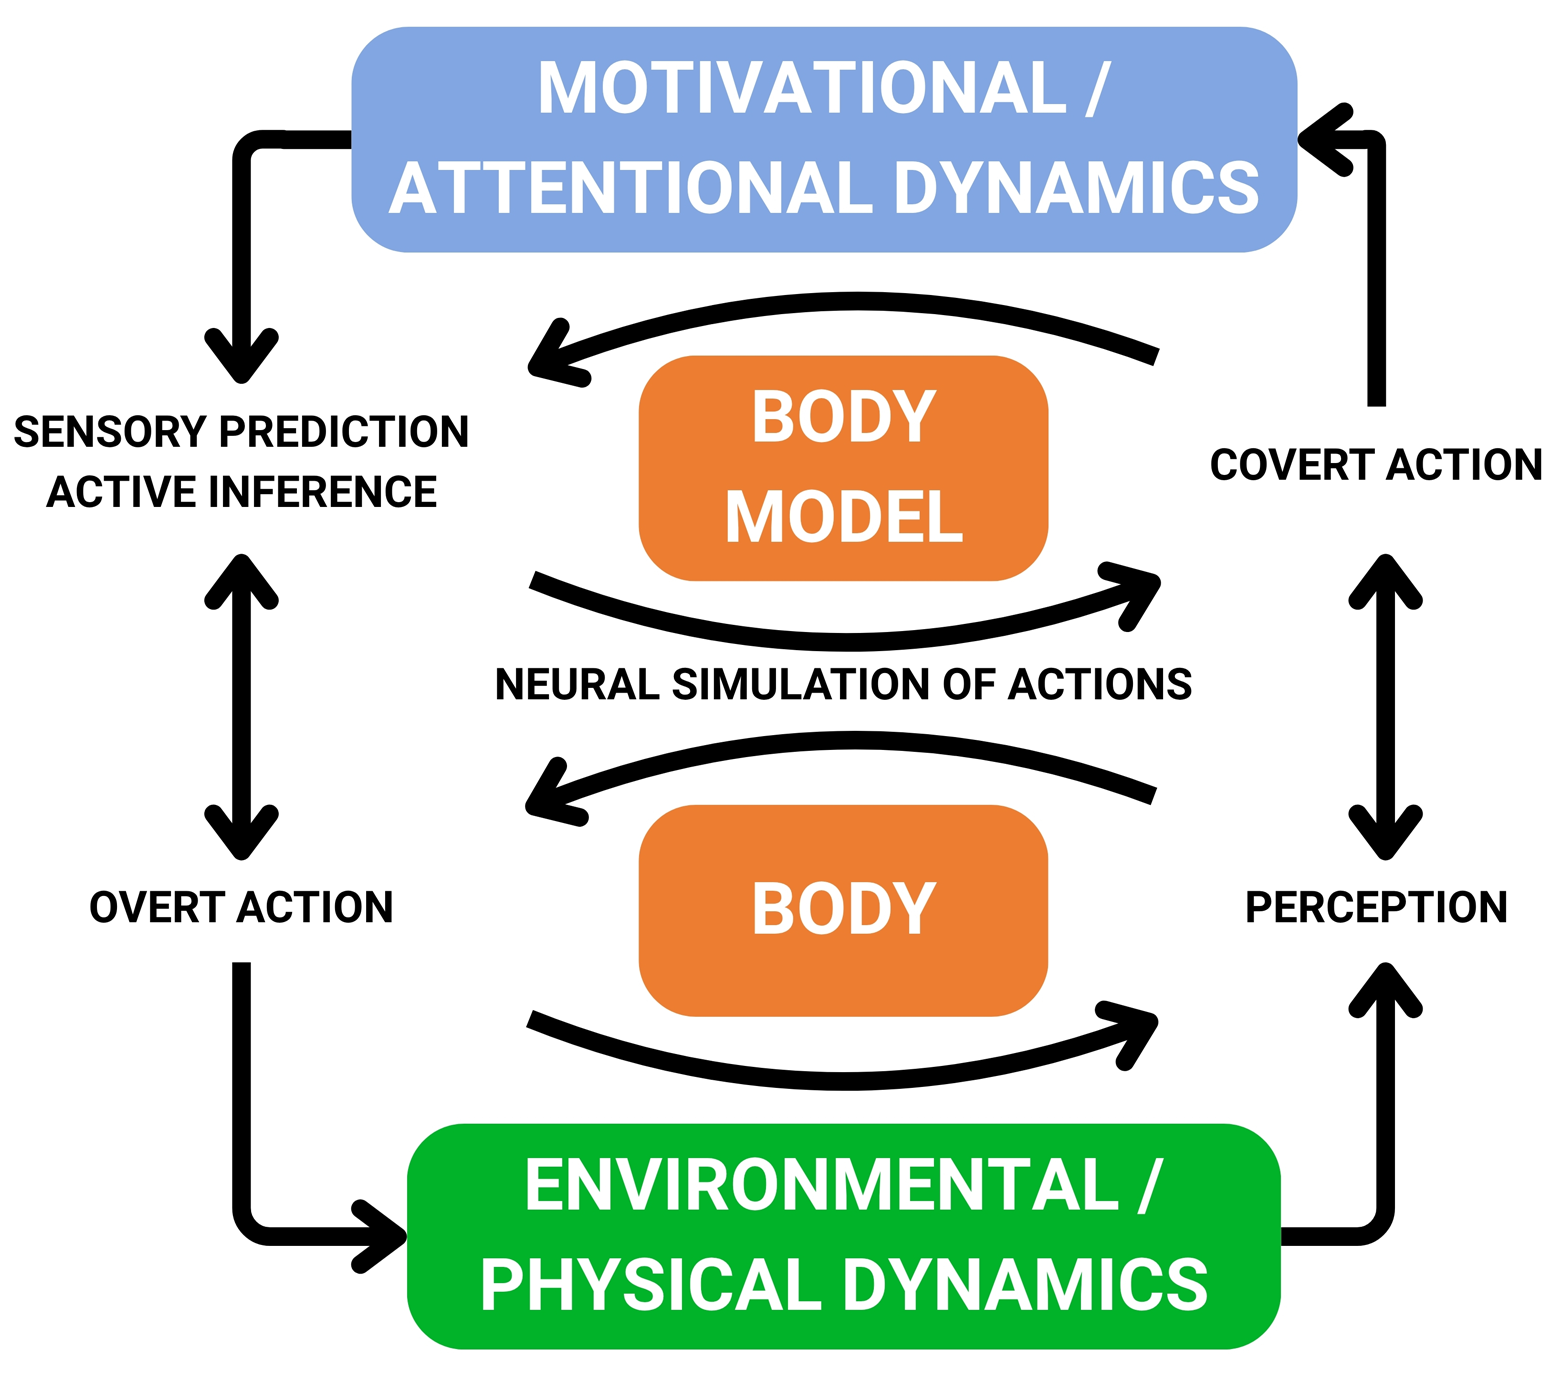
\includegraphics[width=0.62\textwidth,height=0.34\textheight,keepaspectratio]{Introduction/Figures/iseed-coupled-loops.png}
    \caption[Cognition as a system of coupled dynamical loops.]{Cognition as coupled parallel loops, reproduced from \citet{Pasquali2026ISEED} under CC~BY. The lower loop couples body to environmental dynamics through overt action and perception; the upper couples a body model to motivational and attentional dynamics through covert action and sensory prediction.}
    \label{fig:pasquali-iseed-loops}
\end{figure}

The architecture ran on the \emph{ICubHead}, the iCub's actuated head on a stationary 3D-printed upper body, with six degrees of freedom (DoF) in neck and eyes \citep{Pasquali2024ArtificialCognition,Pasquali2025AlwaysOn}. Two eye-mounted RGB cameras gave $640 \times 480$ video at 20~frames per second and an external miniDSP ambiMIK-1 microphone recorded 44.1~kHz stereo audio; the head also has a speaker and LEDs for facial expressions. Only perception and motor control ran on the head itself. Video embedding and memory clustering ran on an external \mbox{workstation} (Intel Core i7 2.6~GHz, 16~GB RAM), linked to the head over the YARP middleware as a distributed, asynchronous network \citep{Metta2006YARP,Pasquali2025AlwaysOn}.

\subsection{The global cognitive loop and modular architecture}
\label{subsec:intro-modular-organization}

The four modules form one continuous perception--action loop in spaces shared with people (Figure~\ref{fig:pasquali-always-on-architecture}): what the robot senses turns its head, and the turn changes what it senses.

\begin{enumerate}
    \item \emph{Multimodal Perception} is the robot's minimal innate equipment for social awareness, modelled on early development: newborns attend to faces, sounds and biological motion, and infants engage in mutual gaze from about three months. Illumination is added to tell moments of the day apart \citep{Pasquali2025AlwaysOn}. From 20~Hz video frames and audio chunks the module extracts five features: visible faces ($F$), people gazing at the robot (mutual gaze), visual motion ($M$), illumination, and right and left audio root-mean-square amplitude ($R, L$). The implementation is deliberately coarse. Faces are counted from a separate object-recognition module's detections. Motion and audio register energy only, without separating biological from other movement or speech from other sound, so the design assumes people produce most of both. Raw audio and video are kept for later encoding.

    \item \emph{Embodied Behavior} steers the head according to an innate \emph{social motive}, modelled on infants' tendency to seek other interactive agents. It tracks a face in view and otherwise alternates between resting and wandering its gaze over random points, both to search for faces and to widen the area it observes \citep{Pasquali2024ArtificialCognition,Pasquali2025AlwaysOn}. The head cannot manipulate objects, so its only actions are gaze shifts that serve exploration. YARP joint states tag every observation with the head posture it was made from.

    \item \emph{Episode Segmentation}, inspired by infants' search for novelty and regularity, cuts the stream into episodes: stretches of time during which the features stay close to their running averages. An \emph{event} is a timestamped snapshot of the synchronised frame and audio chunk, the five features and the joint states; an \emph{episode} is the sequence of events between two boundaries. The module tracks the running mean ($\mu$) and standard deviation ($\sigma$) of $F$, $M$, $R$ and $L$ in the current episode, and an event with $|x_i - \mu_i| > 3\sigma_i$ sets that feature's outlier indicator ($\mathbb{I}_i \in \{0, 1\}$).\footnote{\citet{Pasquali2026ISEED} report the criterion as a deviation of at least twice the modality mean. This account follows \citet{Pasquali2025AlwaysOn}, which specifies the validated segmentation in full and states the three-standard-deviation rule explicitly.} A boundary falls when
    \begin{equation}
        W_F \cdot \mathbb{I}_F + W_M \cdot \mathbb{I}_M + W_{AR} \cdot \mathbb{I}_{AR} + W_{AL} \cdot \mathbb{I}_{AL} \ge 0.5,
        \label{eq:intro-segmentation}
    \end{equation}
    with fixed weights $W_F = 0.5$, $W_M = 0.25$ and $W_{AR} = W_{AL} = 0.125$. Faces carry half the weight, so a person arriving or leaving can close an episode alone. Motion and both audio channels carry the other half and must all be outliers together. This bias toward social events is deliberate. The closed episode is stored in a local SQLite database with its summary statistics and compressed media (.mp4, .wav), and the outlier event that closed it opens the next.

    \item \emph{Implicit Associative Memory} is modelled on infants' earliest memory, which links repeated episodes without recalling any one of them. It provides recognition (is the episode familiar, and to which cluster does it belong?) and temporal expectation (does it fit what usually happens at that time of day?). Both work by learning online as experience arrives and consolidating it offline later.

    Pretrained networks encode each closed episode. SlowFast (ResNet-50, Kinetics-400) maps the video to 400 action-class scores, VGGish maps each audio channel to 128 dimensions, and the channel-averaged audio vector joins the video vector in a 528-dimensional embedding. At the end of each day, or on demand in an induced resting state likened to a power nap, the embeddings are consolidated \citep{Pasquali2025AlwaysOn}. Uniform Manifold Approximation and Projection (UMAP) compresses them to 2D, Hierarchical Density-Based Spatial Clustering of Applications with Noise (HDBSCAN) finds dense clusters of any shape and labels outliers as noise (cluster $-1$), and a grid search picks the hyperparameters that maximise the silhouette score.

    Each new episode is then projected onto the learned manifold as soon as it closes and given a context label ($\ell_t \in \{-1, 0, 1, \dots\}$). After at least a day of operation, the memory also knows which cluster usually occurs in each time window, so it can expect the lively cluster during a midday coffee break and flag a mismatch when the live label differs.
\end{enumerate}

\subsection{Ecological validation and emergent context awareness}
\label{subsec:intro-ecological-validation}

\citet{Pasquali2025AlwaysOn} tested the pipeline in two multi-day deployments in real, unscripted settings:
\begin{itemize}
    \item \emph{Shared office:} Beside the lab's break area, the robot recorded 24 hours over four working days and segmented 449 episodes (Figure~\ref{fig:pasquali-office-validation}). Unsupervised, the memory settled on two clusters (silhouette score 0.69). A \emph{lively} cluster had more faces, mutual gaze, motion and sound, with 91\% of its episodes in the 1--1:30~PM coffee break; episodes between 1 and 2~PM averaged about a minute, against about 25 minutes otherwise. A \emph{calm} cluster held longer episodes of an empty room or quiet desk work. Its episodes were also brighter, which the authors attribute to the wandering gaze settling on the window when no face was in view.
    \item \emph{Conference:} In the Humanoids 2024 demonstration area in Nancy, the robot ran 15 hours over three days and segmented 2,304 shorter episodes (mean 15~s). Lively and calm clusters formed again (silhouette score 0.67); 61\% of lively episodes fell between 2 and 4~PM, around the afternoon coffee break, and 75\% of calm ones during talk sessions.
    \item \emph{Both venues:} One memory built from both datasets told the venues apart with 98.7\% accuracy and kept the lively--calm split within each.
\end{itemize}

\begin{figure}[tbp]
    \centering
    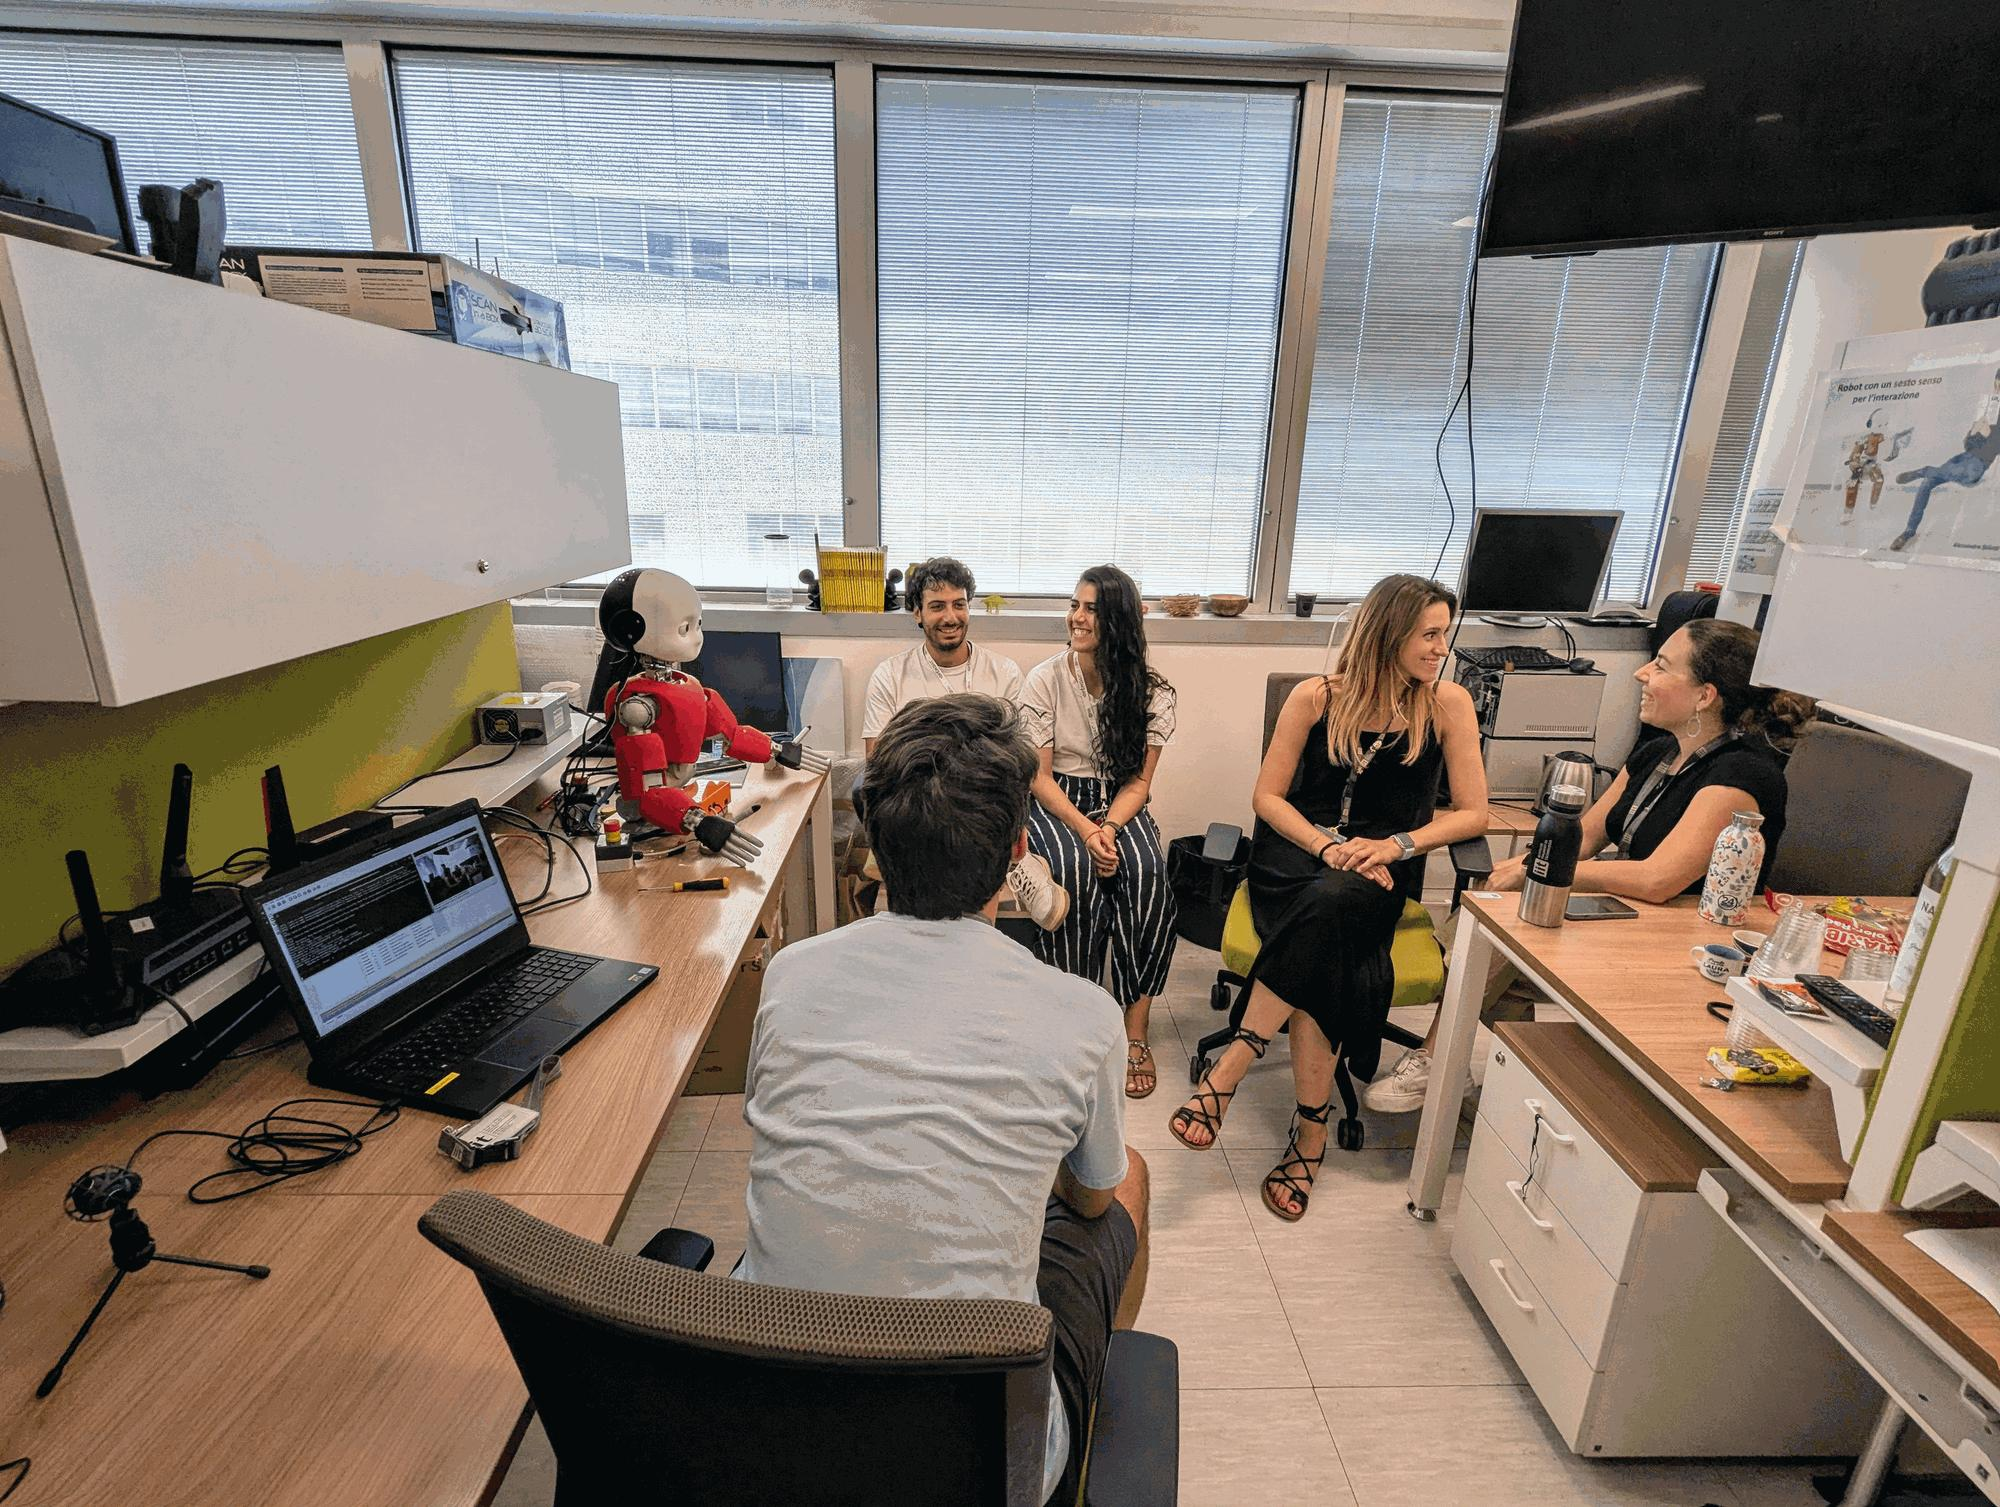
\includegraphics[width=0.88\textwidth,height=0.38\textheight,keepaspectratio]{Introduction/Figures/office-validation.png}
    \caption[Shared-office validation of the always-on architecture.]{Shared-office validation of the always-on cognitive architecture. The ICubHead was positioned beside a break area \citep{Pasquali2025AlwaysOn}.}
    \label{fig:pasquali-office-validation}
\end{figure}

\citet{Pasquali2026ISEED} then asked whether the clusters were stable enough to support expectation. Lacking external labels, they scored the memory against the agent's own goal of internal consistency: recognition accuracy (the same label in real time and after consolidation), temporal stability (the same label across days) and expectation consistency (the live context matching the one prior experience made most likely at that hour). In the office every measure improved with experience, recognition accuracy from 0.23 to 0.93 and expectation consistency from 0.24 to 0.96. At the conference the three measures diverged. Recognition (0.83, then 0.73) and stability (around 0.78) stayed above 0.7, but expectation consistency fell to 0.26 and then 0.08. A memory built from first-person experience inherits the regularity of the place that supplied it, and an exhibition hall with shifting schedules supplies little. A drive that must time its requests to human availability faces the same limit.

Dario Pasquali later refactored the architecture to run online (Section~\ref{subsec:developmental-context-coupling}). VideoMAE replaced SlowFast, which cut latency and brought context inference into the live control path. The memory now has an online hippocampal path for rapid encoding and a neocortical module for long-term consolidation, so experience accumulates without pausing capture. This removes a limitation \citet{Pasquali2025AlwaysOn} name themselves: recognition waited for an episode to close, so the context label lagged behind any interaction under way.

\section[An embodied behaviour architecture for drive-guided action]{An embodied behaviour architecture\\for drive-guided action}
\label{sec:intro-embodied-behaviour-architecture}

A value system has no effect unless it can reach behaviour, and the inherited \emph{Embodied Behavior} module offered no interface for it. This thesis therefore replaces that module with a behaviour layer through which any signal from the cognitive architecture, a motivational state or a recognised context, can change whom the robot attends to and what it says. Choosing an interaction partner requires telling people apart, and the inherited perception only counted faces, so I rewrote the vision module to track each person as an individual (Section~\ref{sec:multimodal-perception}). Attentional control selects whom to engage from perceptual evidence and learned per-person affinity, while executive control reads the robot's internal state to set the priority of regulatory behaviour. The resulting policy separates four kinds of behaviour by their trigger: reactive (a person greets the robot), proactive (a salient, eligible person is in view), expressive (the robot's hunger state) and remote (a hunger-state change, reported over Telegram). Apart from the vision module, perception, segmentation and memory still come from the surrounding always-on architecture.

The same layer supplies the action-selection loop that \citet{Pasquali2025AlwaysOn} found missing and that \citet{Pasquali2026ISEED}, whose validation was achieved \emph{before} closing the action loop, place on their roadmap. An internal drive sets executive priority once an interaction starts, and the outcome of each interaction feeds back through affinity into the eligibility governing later target selection. None of these interfaces is specific to one need: a drive enters the layer by publishing a state the executive controller can read and an outcome from which affinity can be learned, so curiosity or fatigue would travel the same path as hunger.

\section[Homeostasis and the synthetic orexigenic drive]{Homeostasis and the\\synthetic orexigenic drive}
\label{sec:intro-homeostasis-drive}

\citet{Pasquali2025AlwaysOn} end their account by arguing that deciding what belongs in memory first requires defining what matters to the agent, and they name energy among the internal drives that could serve that role. Energy is the value installed on the new layer.

A social robot that runs out of energy stops being a social robot: face detection, dialogue and memory consolidation all stop with it. A review of long-term HRI studies finds that recharging which takes too long or comes at the wrong time constrains what the robot can do \citep{Matheus2025LongTerm}, and in a three-week office deployment it degraded the service users expected \citep{Deshmukh2018Recharging}. An always-on architecture, which acquires its knowledge through uninterrupted immersion in a shared space, is especially exposed: every shutdown cuts the stream of experience the system learns from.

The conventional response treats energy as telemetry: a battery percentage is monitored, a threshold fires, and the robot either docks autonomously or waits for an operator to notice. Both options take the robot out of the interaction and give the people around it no role, although in a shared office or an exhibition hall those people already pay attention to it. With the new behaviour layer in place, the robot can ask them for energy instead of managing it silently.

Animals solved the problem of keeping a draining resource topped up long ago. Homeostasis is the self-regulating process that keeps an organism's internal environment within viable bounds while the outside world changes \citep{Cannon1929Homeostasis}. In a homeostatic system a deficit reorganises what the animal attends to and what it does next. Hunger narrows attention toward food-related cues \citep{Petzschner2021Interoception} and raises the priority of foraging over other pursuits. When several such variables compete, their relative urgency decides behaviour \citep{Hulme2019HomeostaticControl,Rosado2022DriveCompetition}.

The mechanism proposed here is a synthetic \emph{orexigenic homeostatic drive}. It rests on an energy resource that drains over time and with each social action the robot takes. When the resource leaves its preferred range, the gap acts as a regulatory error that reorders the priority of candidate actions. The term \emph{orexigenic} names the role the variable plays: as the deficit grows, more of the robot's behaviour is directed toward getting fed. At critical depletion, feeding requests take precedence over ordinary social dialogue.

\citet{Pasquali2026ISEED} set a stricter test, causal grounding. A designer can impose constraints that reproduce value-consistent behaviour without the agent ever owning a value, so a value counts as grounded only if it forms through the agent's own experience. The orexigenic drive passes only part of that test (Section~\ref{sec:disc-loop-closure}).

Because the behaviour available to a social robot is social, a deficit that recruits behaviour seeks replenishment through the people present, and energy maintenance becomes an HRI problem: as the internal state approaches its critical region, the robot asks for help in speech, or over Telegram when nobody is present, before depletion ends the interaction. Depending on people does not weaken autonomy, which here includes deciding when and how to seek help; a robot that cannot charge itself gains nothing by running down without asking.

\section{Contributions}
\label{sec:intro-contributions}

\paragraph{An adaptable embodied behaviour architecture.}
A behaviour layer replaces the fixed policy of the original \emph{Embodied Behavior} module, keeps per-person memory across sessions and lets an internal state reshape attention, interaction eligibility and dialogue within the always-on perception--action loop. A rewritten vision module supplies the per-person observations it needs.

\paragraph{An operational value system.}
A synthetic orexigenic variable is installed on that layer. Its distance from the preferred range decides how much an event or action matters for regulation.

\paragraph{Action selection and loop closure.}
The layer coordinates reactive response, proactive initiation, embodied expression and remote contact according to the robot's social perception and internal need, with feeding requests taking priority in critical deficit. Energy regulation becomes a traceable HRI process: the robot asks for help, and a measurable recovery shows whether the help arrived.

\paragraph{Outcome-grounded social adaptation.}
Homeostatic affinities, learned per person, record who has fed the robot and bias later approaches, so regulatory outcomes enter social memory without blocking the escalation of critical requests.

\section{Research questions}
\label{sec:intro-research-questions}

The thesis asks whether, once a behaviour layer is added to the always-on architecture, a single measurable internal drive can change both how iCub acts toward people and what it learns from them. Showing that the robot can say it is hungry would validate neither the drive nor the layer that carries it. The criterion is whether the drive, acting through the behaviour architecture, changes action selection and produces recovery in a closed loop that can be traced in the logs. Purely reactive systems and scripted hunger displays fail this test, because no internal state changes what they select. Each link in the chain must stay visible in the data: detecting a deficit must lead to recovery-oriented action, that action must draw an observable response, the response must produce replenishment, and replenishment must alter later caregiver selection.

Regulatory effectiveness and human interpretation can still come apart: a robot might restore its energy efficiently while communicating poorly, or appear expressive while rarely getting fed. I therefore treat control validity, recovery success, adaptive memory and user perception as four levels of evidence, none of which can stand in for another, and ask one question per level.

\begin{description}
    \item[RQ1.] Does the orexigenic drive fulfil the core functions of classical homeostasis: internal monitoring, deficit detection, deficit-to-action conversion, and a change in how far interactions progress once a threshold is crossed?
    \item[RQ2.] In an always-on social robot, does expressing an orexigenic deficit draw recovery-oriented help from people, and does that help restore the energy resource reliably, after every request?
    \item[RQ3.] Does the robot's adaptive regulatory memory encode observed participant behaviour, and is that learned state subsequently expressed at the eligibility gate that governs proactive approach?
    \item[RQ4.] In what ways does the behavioural expression of the orexigenic drive shape users' perception of the robot as a socially embedded and natural interaction partner?
\end{description}

\section{Structure of the thesis}
\label{sec:intro-thesis-structure}

Chapter~\ref{chap:state-of-the-art} reviews the prior work on which the design rests. Chapter~\ref{chap:methodology} describes the architecture layer by layer and ends with the deployment protocol and statistical analysis. Chapter~\ref{chap:results} reports the deployment against each research question in turn, Chapter~\ref{chap:discussion} interprets the results and states their limits, and Chapter~\ref{chap:conclusion} answers the research questions and points to future work, mostly on the memory side of the always-on architecture. Four appendices give the language-model prompts, questionnaire items, fitted feeding model and an implementation reference.
